\chapter{Uitbreidingen van de Unipept command-line interface}
\chaptermark{Unipept CLI}
\label{chap:cli}

De Unipept command-line interface\cite{toonthesis} (CLI) is een verzameling van
tools geschreven door Toon Willems gedurende zijn masterthesis in het
academiejaar 2013-2014. Deze interface is ontwikkeld in Ruby en maakt gebruikt
van de Unipept HTTP API.\cite{Unipeptapi}.

Gedurende de case study in \Cref{chap:casestudy} werd de CLI zeer intensief
gebruikt. Door dit intensief gebruik zijn enkele fouten en problemen naar boven
gekomen. In dit hoofdstuk bespreken we, na een korte inleiding tot de CLI, de
oorzaak van die problemen en geven we ook aan hoe we ze hebben opgelost.

\section{Inleiding tot de Unipept CLI}
De Unipept command-line interface wrapt de vijf basismethodes van de 
Unipept webservices\cite{Unipeptapi} in een command-line interface. De werking 
van deze commando's staat geillustreerd in \Cref{fig:apiworkflow} op 
\cpageref{fig:apiworkflow}.

\begin{itemize}
\item \textbf{\texttt{pept2prot}:} geeft een lijst van UniProt entries 
die een opgegeven peptide bevatten;
\item \textbf{\texttt{pept2taxa}:} geeft een lijst van taxa geëxtraheerd uit 
UniProt entries die de opgegeven peptide bevatten;
\item \textbf{\texttt{pept2lca}:} geeft de taxonomische lowest common ancestor 
voor een gegeven tryptische peptide;
\item \textbf{\texttt{taxa2lca}:} geeft de taxonomische lowest common ancestor 
voor een gegeven lijst van taxon identifiers;
\item \textbf{\texttt{taxonomy}:} geeft taxonomische informatie voor een 
gegeven taxon identifier.
\end{itemize}

\begin{figure}
	\centering
	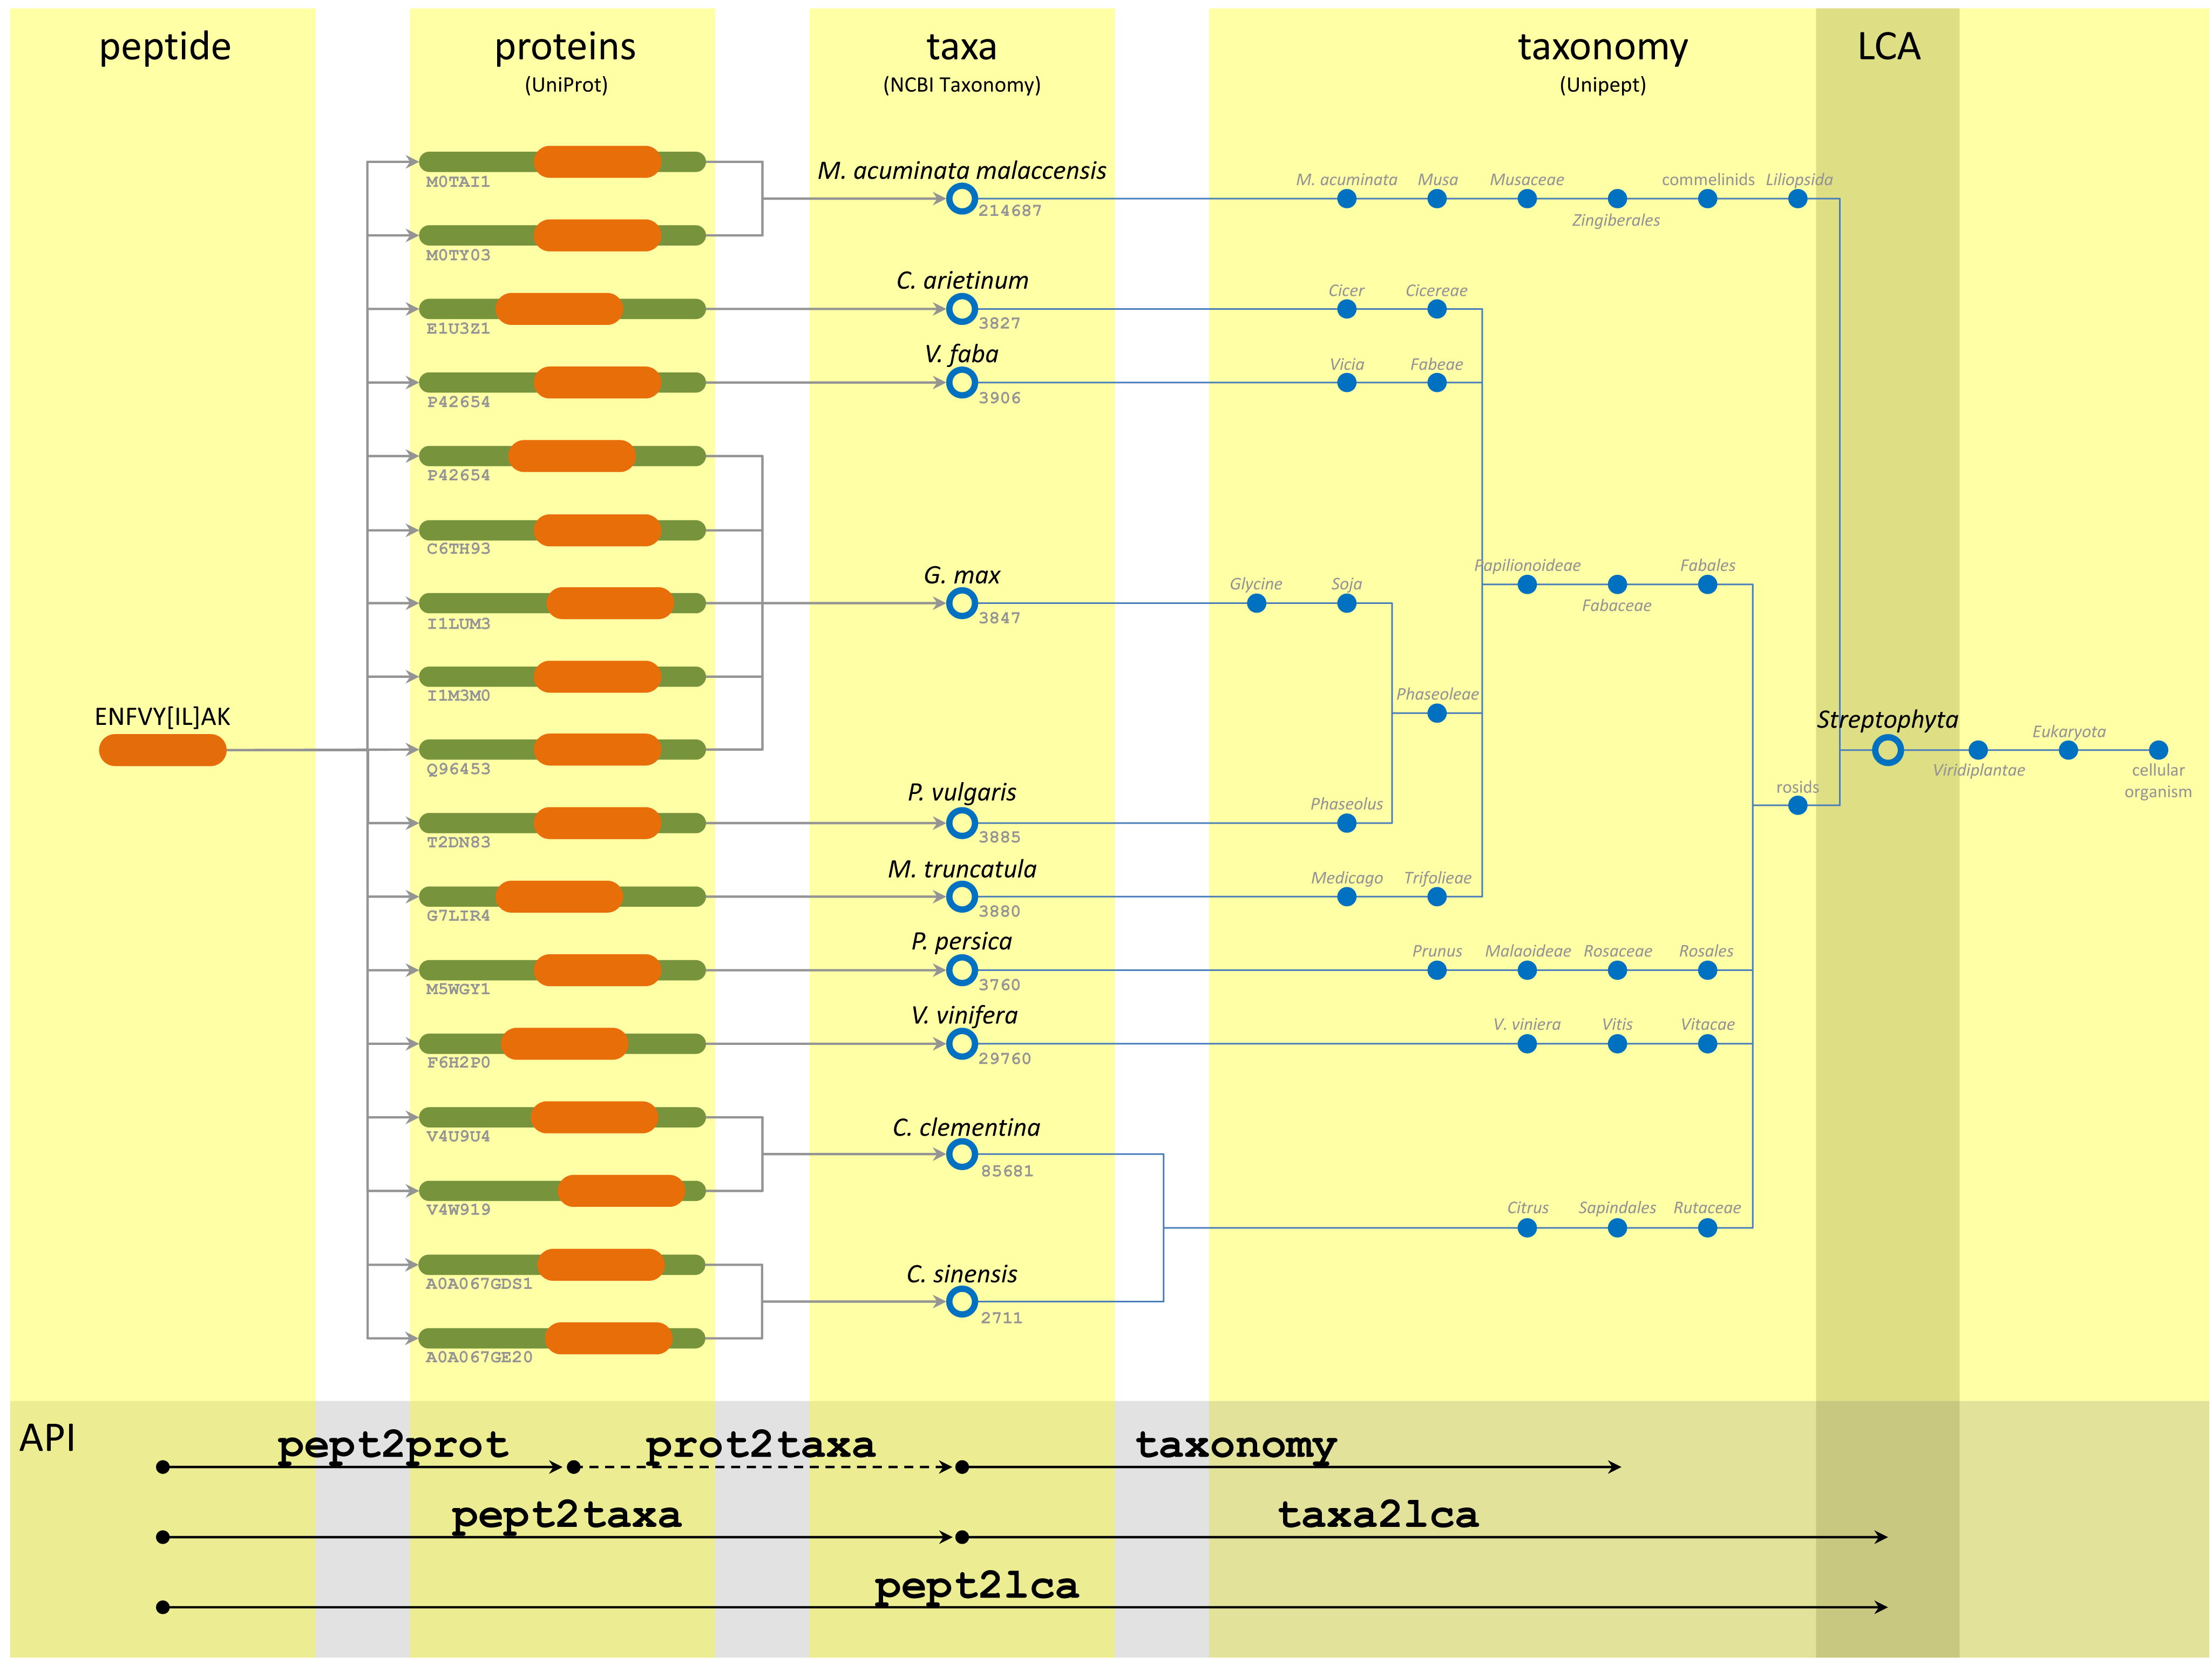
\includegraphics[width=0.8\textwidth]{includes/apiworkflow}
	\caption{Illustratie van de vijf basiscommando's aangeboden door de Unipept 
	webservices.}
	\label{fig:apiworkflow}
\end{figure}

Voor de CLI kan gebruikt worden, moet deze eerst lokaal geinstalleerd worden. 
Aangezien alle commando's geïmplementeerd zijn in Ruby moet eerst een Ruby 
environment worden geïnstalleerd. De CLI kan daarna eenvoudig geïnstalleerd 
worden met het het commando \texttt{gem}, de interne Ruby Package manager. De 
broncode van de CLI kan gevonden worden op de publieke Unipept-cli repository, 
\url{https://github.com/unipept/unipept-cli}.

\begin{lstlisting}
$ gem install unipept
Successfully installed unipept-0.6.4
1 gem installed
Installing ri documentation for unipept-0.6.4...
Installing RDoc documentation for unipept-0.6.4...
\end{lstlisting}

Na de installatie van de Unipept gem is het \texttt{unipept}-commando 
beschikbaar. De namen van de methodes van de webservices komen 
overeen met de naam van de subcommandos van het Unipept CLI-commando. De 
helpfuncties en extra opties kunnen dan worden opgevraagd via 
de \texttt{--help} vlag:

\begin{lstlisting}
$ unipept --help

COMMANDS
  config
  help          show help
  pept2lca      Give lowest common ancestor for given peptide
  pept2prot     Give protein information for given peptides
  pept2taxa     Single Peptide Search
  taxa2lca      Give lowest common ancestor for taxon ids
  taxonomy      Give NCBI taxonomy information on given input taxon ids

OPTIONS
  -f --format     output format (available: json,csv,xml) (default: csv)
  -h --help       show help for this command      
     --host       Override host setting
  -i --input      input file
  -o --output     output file
  -q --quiet      don't show update messages
  -v --version    print version
\end{lstlisting}

Zoals eerder vermeld steunt de CLI op de Unipept webservices. Vooraleer de 
commando's kunnen worden uitgevoerd moet dus een API server worden opgegeven 
via de \texttt{--host} vlag. Deze kan ook als standaardserver worden ingesteld 
via het \texttt{config} subcommando, zodat de \texttt{--host} vlag niet telkens 
opnieuw hoeft worden te meegegeven.

\begin{lstlisting}
$ unipept --host 'api.unipept.ugent.be' pept2lca ENFVYIAK
peptide,taxon_id,taxon_name,taxon_rank
ENFVYIAK,35493,Streptophyta,phylum
$ unipept config host='api.unipept.ugent.be'
$ unipept pept2lca ENFVYIAK
peptide,taxon_id,taxon_name,taxon_rank
ENFVYIAK,35493,Streptophyta,phylum
\end{lstlisting}

Het voorgaande voorbeeld toont hoe het \texttt{unipept pept2lca}-commando wordt 
aangeroepen voor de peptide \texttt{ENFVYIAK}. We kunnen ook alle eiwitten 
voor deze peptide opvragen via \texttt{unipept pept2prot}:

\begin{lstlisting}
$ unipept pept2prot MVNENTR
peptide,uniprot_id,taxon_id
ENFVYIAK,Q96453,3847
ENFVYIAK,C6TH93,3847
ENFVYIAK,P42654,3906
ENFVYIAK,M0TY03,214687
ENFVYIAK,A0A067GDS1,2711
ENFVYIAK,C6TM63,3847
...
\end{lstlisting}

\section{Verwerken van FASTA files}
Een recente toevoeging aan de commandolijn is de verwerking van FASTA files.
Door deze toevoeging kunnen FASTA bestanden meegegeven worden als invoerbestand
aan de commando's. Bij de resultaten worden de resultaten dan ook gegroepeerd
onder hun overeenkomstige FASTA header. Tijdens de case study uit vorig
hoofdstuk bleek dat FASTA files niet altijd correct verwerkt werden. Wanneer we
dezelfde peptide toevoegen onder verschillende FASTA headers, kregen we in de
output steeds enkel de laatst voorgekomen FASTA header te zien. Ook de eerdere
FASTA headers werden bij die peptides vervangen door de laatste. Volgend
voorbeeld illustreert het probleem:

\begin{lstlisting}
$ cat data/IITHPNFNGNTLDNDIMLIK 
>a|1
IITHPNFNGNTLDNDIMLIK
>b|2
IITHPNFNGNTLDNDIMLIK

$ unipept pept2lca -i data/IITHPNFNGNTLDNDIMLIK 
fasta_header,peptide,taxon_id,taxon_name,taxon_rank
>b|2,IITHPNFNGNTLDNDIMLIK,9823,Sus scrofa,species
>b|2,IITHPNFNGNTLDNDIMLIK,9823,Sus scrofa,species

$ unipept pept2prot -i data/IITHPNFNGNTLDNDIMLIK
fasta_header,peptide,uniprot_id,taxon_id
>b|2,IITHPNFNGNTLDNDIMLIK,P00761,9823
>b|2,IITHPNFNGNTLDNDIMLIK,C5IWV5,9823
>b|2,IITHPNFNGNTLDNDIMLIK,F1SRS2,9823
>b|2,IITHPNFNGNTLDNDIMLIK,P00761,9823
>b|2,IITHPNFNGNTLDNDIMLIK,C5IWV5,9823
>b|2,IITHPNFNGNTLDNDIMLIK,F1SRS2,9823
\end{lstlisting}

We zien dat de fasta header \texttt{b|2} wordt toegevoegd voor alle resultaten 
van de peptide \texttt{IITHPNFNGNTLDNDIMLIK}, ook wanneer de \texttt{a|1} de 
correcte header is, komt er header \texttt{b|2} te staan.

De oorzaak van het probleem lag bij de mapping van de FASTA headers. Het 
verwerken van het FASTA gedeelte gebeurt volledig aan de kant van de gebruiker. 
De server is dus nooit op de hoogte van het bestaan van de 
FASTA headers. Daarom 
moeten de command-line tools zelf een mapping bijhouden van peptides op FASTA 
headers. Daarna worden de peptides zonder headers naar de server gestuurd en 
worden de fasta headers bij het antwoord van de server terug op de peptides 
gemapt.

De onderstaande code illustreert hoe deze mapping gebeurt:

\begin{lstlisting}[language=Ruby]
# Input: een fastafile, genaamd `input` en een `block`

# Slaat de eerste header op in een tijdelijke variabele
fasta_header = input.next

# Breekt de invoer op in stukken (= batches) van 200
input.slice(200) do |batch|
  # Maak een hash aan die binnen een batch een peptide op een fasta header mapt
  fasta_mapper = {}
  
  # Itereert over de lijnen in 1 batch
  j = 0
  while j < batch.size
    # Als de huidige lijn start met een > is deze een fasta header
    if batch[j].start_with? '>'
      # Overschrijf de fasta_header variabele met de huidige fasta header
      fasta_header = batch[j]
    else
      # Voeg de fasta header toe aan de map
      fasta_mapper[batch[j]] = fasta_header
    end
    j += 1
  end
  
  # Verwijder de fasta headers uit de batch
  batch -= fasta_mapper.values.uniq
  
  # Stuur de batch zonder fasta headers naar de API ter verwerking
  block.call(batch, fasta_mapper)
end
\end{lstlisting}

De oorzaak van het probleem lag op regel 9 van bovenstaande code. Door één
enkele FASTA header op één peptide te mappen wordt de FASTA header overschreven
wanneer er meerdere gelijke peptides binnen één batch aanwezig zijn. Als we er
het voorbeeld van hierboven bijnemen, dan bevat de \texttt{fasta\_mapper} na 
het
overlopen van de eerste FASTA groep onder header \texttt{a|1} een mapping van
\texttt{'IITHPNFNGNTLDNDIMLIK' => 'a|1'}, maar wanneer de tweede FASTA groep
gelezen is, wordt de waarde overschreven naar \texttt{b|2}.

Bij het uitschrijven werd er per peptide die de API die als resultaat door de 
API wordt teruggeven, een mapping 
gemaakt van peptide naar FASTA header. Aangezien de FASTA headers van 
peptides in bepaalde gevallen overschreden werden, werd de mapping soms fout 
gemaakt.

Om dit probleem op te lossen zouden we een mapping kunnen bijhouden van één
peptide op meerdere fasta headers. Bij de output kunnen we dan berekenen welke
header we moeten nemen afhankelijk van het aantal keer die peptide al is
uitgeschreven. Na implementatie bleek de uitvoeringstijd echter veel trager
(grootteorde 20) en veel meer belastend voor zowel de processor als het geheugen
dan gewenst (ook al was de uitvoer correct).

Het mappen van peptides op hun FASTA header is dus geen goede oplossing voor
genoemd probleem. In plaats van te werken met dit soort mapping kunnen we ook 
een lijst
bijhouden van een inputpaar, bestaande uit FASTA header en peptide. De code om
dit te bereiken ziet er als volgt uit:

\begin{lstlisting}[language=Ruby]
# Input: een fastafile, genaamd `input` en een `block`

# Slaat de eerste header op in een tijdelijke variabele
fasta_header = input.next

# Breekt de invoer op in stukken (= batches) van 200
input.slice(200) do |batch|
  # Maak een hash aan die binnen een batch een peptide op een fasta header mapt
  fasta_input = []
  
  # Gebruik een Set om de peptides op te slaan zodat we niet dezelfde peptide 2 
  # keer naar de server sturen 
  newsub = Set.new
  
  # Itereert over de lijnen in 1 batch
  sub.each do |s|
    s.chomp!
    if s.start_with? '>'
      # Sla de huidige fasta_header op in een tijdelijke variabele
      fasta_header = s
    else
      # Voeg het inputpaar toe aan de lijst
      fasta_input << [fasta_header, s]
      newsub << s
    end
  end
  
  # Stuur de batch zonder fasta headers naar de API ter verwerking
  block.call(newsub, fasta_input, ...)
end
\end{lstlisting}

Op deze manier hebben we (opnieuw aan de hand van het voorbeeld) de volgende 
variabelen: \texttt{newsub} die één element bevat: 
\texttt{IITHPNFNGNTLDNDIMLIK}, en \texttt{fasta\_input} die de volgende lijst 
bevat: \texttt{[(a|1, IITHPNFNGNTLDNDIMLIK), (b|2, IITHPNFNGNTLDNDIMLIK)]}. 
\texttt{newsub} wordt dan naar de server gestuurd ter analyse.

Om de mapping terug te maken van peptide naar fasta header bekijken we eerst de
structuur van resultaten voor de peptide. Commando's zoals \texttt{pept2lca}
geven per invoerpeptide één resultaat terug. Commando's zoals \texttt{pept2prot}
kunnen echter meerdere resultaten teruggeven per peptide:

\begin{lstlisting}
$ curl `api.unipept.ugent.be/api/v1/pept2lca.json?input[]=IITHPNFNGNTLDNDIMLIK`
[
  {
    "peptide": "IITHPNFNGNTLDNDIMLIK",
    "taxon_id": 9823,
    "taxon_name": "Sus scrofa",
    "taxon_rank": "species"
  }
]

$ curl `api.unipept.ugent.be/api/v1/pept2prot.json?input[]=IITHPNFNGNTLDNDIMLIK`
[
  {
    "peptide": "IITHPNFNGNTLDNDIMLIK",
    "uniprot_id": "P00761",
    "taxon_id": 9823
  },
  {
    "peptide": "IITHPNFNGNTLDNDIMLIK",
    "uniprot_id": "F1SRS2",
    "taxon_id": 9823
  },
  {
    "peptide": "IITHPNFNGNTLDNDIMLIK",
    "uniprot_id": "C5IWV5",
    "taxon_id": 9823
  }
]
\end{lstlisting}

Ook bij het uitschrijven voeren we een verandering door. In de oude code werd 
de lijst van resultaten overlopen en werd op elk resultaat een FASTA header 
gemapt. Met de nieuwe code is dit niet langer mogelijk aangezien we de 
peptides die binnen één batch meerdere keren voorkomen maar één keer naar de 
server 
sturen. We moeten hier dus de \texttt{fasta\_input} lijst overlopen 
en daar de resultaten op mappen. Dit gebeurt als volgt:

\begin{lstlisting}[language=Ruby]
# Hervorm de resultaten van [{key1: value1, key2: value2, ...}]
# naar {value1 => {key1: value1, key2: value2, ...}}
data_dict = {}
data.each do |d|
  data_dict[d.values.first.to_s] ||= []
  data_dict[d.values.first.to_s] << d
end

# Itereer over de invoer
fasta_input.each do |input_pair|
  fasta_header, id = input_pair

  # Haal het resultaat voor het id op (indien die er is)
  unless data_dict[id].nil?
    data_dict[id].each do |r|
      csv << ([fasta_header] + r.values).map { |v| v == "" ? nil : v }
    end
  end
end
\end{lstlisting}

Aangezien één peptide meerdere resultaten kan hebben, moeten we de lijst van de
resultaten eerst hervormen, zoals gebeurt in regel 3 tot 7 van bovenstaande
code. Dit is een preprocessing stap die ervoor zorgt dat we de bijhorende
resultaten van een peptide eenvoudig op kunnen halen zonder telkens de hele
resultatenlijst af te moeten lopen. Op regel 14 doen we ook nog een 
extra check
of er wel degelijk een resultaat is voor de ingevoerde peptide. Het is
namelijk mogelijk dat een peptide geen resultaat oplevert omdat hij niet gekend
is door Unipept.

Deze aanpak heeft (naast correcte resultaten) een aantal voordelen ten opzichte
van de oude. Zo worden peptiden die meerdere keren voorkomen binnen een batch
maar één keer naar de server gestuurd ter analyse. Een tweede voordeel is dat
hiermee een probleem met het \texttt{taxonomy}-commando is opgelost. De API
geeft bij dit commando namelijk maar één resultaat terug wanneer hetzelfde 
taxon vaker worden verstuurd. Aangezien de resultaten nu worden overlopen aan de
hand van de invoer en niet aan de hand van de resultaten zelf zal de CLI altijd 
evenveel resultaten opleveren als er invoerlijnen zijn.

De vraag is natuurlijk of de code nog steeds even performant is als (of
performanter dan) de oude code, en niet dezelfde problemen vertoont als de
vorige oplossing. Dit onderzoeken we in volgende sectie, waar we ook meteen een
onderzoek voeren naar de optimale \texttt{batch size} parameters voor de
verschillende methoden.

\section[Bepalen van de optimale batch size voor de Unipept CLI]{Bepalen van de 
optimale batch size voor de Unipept CLI \sectionmark{Bepalen van optimale batch 
size}}
\sectionmark{Bepalen van optimale batch size}

De CLI stuurt niet alle data in één keer door naar de API. Het zou namelijk
problemen opleveren als er meer data zou worden doorgestuurd dan de server in
één keer kan verwerken, met fouten in de server tot gevolg. We moeten ook in het
achterhoofd houden dat alle data over het netwerk verstuurd moet worden en dat
er ook nog verwerking nodig is langs de kant van de client. De oplossing
hiervoor is om de invoerdata op te delen in stukken, en die stuk voor de stuk
naar de server te sturen om die sequentieel te verwerken. Zo wordt het netwerk
niet overbelast door grote hoeveelheden data en moeten de server en client niet
alle data in één keer bijhouden en verwerken. De grootte van de blokken (of
batches) waarin de data wordt opgedeeld, wordt \texttt{batch size}, of de
batchgrootte genoemd.

Verschillende commando's hebben ook verschillende verwerkingstijden en 
verschillende groottes van resultaten. Het \texttt{pept2lca} commando geeft 
bijvoorbeeld hoogstens één resultaat per peptide, maar voor diezelfde peptide 
kan \texttt{pept2prot} duizenden resultaten teruggeven.

Het komt er dus op neer om een optimale batchgrootte te vinden die voor een 
balans zorgt tussen de data die over het netwerk verstuurd kan worden, de data 
de server kan verwerken en de data die de client kan verwerken. De parameter 
moet daarenboven ook commando-afhankelijk zijn.

Om die parameter te bepalen werden enkele tijds- en CPU-metingen, waarbij de 
batchgrootte werd gevarieerd. Voor commando's die één resultaat per peptide 
teruggeven, werd het commando \texttt{pept2lca} gebruikt met batchgroottes 10, 
100, 1000 en 10000. Voor commando's die meerdere resultaten teruggeven, werd 
\texttt{pept2prot} gebruikt met batchgroottes 5 en 10. Alle testen werden 5 
keer herhaald per batchgrootte. Als invoer werd een dataset gebruikt die 
ongeveer 72000 peptides bevat.

\begin{table}
    \caption{Benchmarking van \texttt{pept2lca} met verschillende 
    batchgroottes}
    \label{tbl:clibenchmark}
    \begin{subtable}{.45\linewidth}
        \centering
        \caption{Oude code}
        \begin{tabular}{rll}
            \toprule 
            Batchgrootte & Tijd (s) & CPU  \\
            \midrule
            10           & 8.9184   & 66\% \\
            100          & 3.4326   & 72\% \\
            1000         & 2.7184   & 81\% \\
            10000        & 4.551    & 87\% \\
            \bottomrule
        \end{tabular}
    \end{subtable}
    \begin{subtable}{.45\linewidth}
        \centering
        \caption{Nieuwe code}
        \begin{tabular}{rll}
            \toprule 
            Batchgrootte & Tijd (s) & CPU  \\
            \midrule
            10           & 8.6656   & 69\% \\
            100          & 3.4776   & 70\% \\
            1000         & 2.9128   & 81\% \\
            10000        & 5.0994   & 82\% \\
            \bottomrule
        \end{tabular}
    \end{subtable}
    \\
    \\
    \caption{Benchmarking van \texttt{pept2prot} met verschillende 
    batchgroottes}
    \begin{subtable}{.45\linewidth}
        \centering
        \caption{Oude code}
        \begin{tabular}{rll}
            \toprule 
            Batchgrootte & Tijd (u) & CPU  \\
            \midrule
            2            & 6:24.24 & 98\% \\
            5            & 5:28.35 & 99\% \\
            10           & 7:35.05 & 99\% \\
            \bottomrule
        \end{tabular}
    \end{subtable}
    \begin{subtable}{.45\linewidth}
        \centering
        \caption{Nieuwe code}
        \begin{tabular}{rll}
            \toprule 
            Batchgrootte & Tijd (u) & CPU  \\
            \midrule
            2            & 6:35.29 & 99\% \\
            5            & 5:34.94 & 99\% \\
            10           & 7:27.31 & 99\% \\
            \bottomrule
        \end{tabular}
    \end{subtable}
\end{table}

Aangezien we, zoals beschreven in vorige sectie, wijzigingen hebben aangebracht 
in de command-line code is het interessant om de benchmarks ook op de oude code 
te laten lopen en zo in te schatten of de nieuwe code nog even performant is. 
De resultaten van deze benchmarks zijn te vinden in \Cref{tbl:clibenchmark} op 
\cpageref{tbl:clibenchmark}. Uit deze tests kunnen we besluiten dat een grotere 
batchgrootte niet altijd beter is. 

Bij het \texttt{pept2lca} commando zakt de uitvoeringstijd steeds naarmate de
batchgrootte groter wordt, tot en met een batchgrootte van 1000. Vanaf die
batchgrootte stijgt de uitvoeringstijd weer. De CPU-belasting neemt wel toe
naarmate de batchgrootte groter wordt. De optimale batchgrootte zou hier dus
1000 zijn.

Bij de benchmarks voor \texttt{pept2prot} zien we een minimum uitvoeringstijd
bij batchgrootte 5. Het CPU-gebruik ligt in alle gevallen tegen het maximum.

Als laatste zien we dat de nieuwe code voor FASTA files op alle vlakken zeer
gelijkaardig presteert als de oude code. Bovendien is de nieuwe code ook
volledig correct.

In de toekomst kan het interessant zijn om de batchgrootte te laten afhangen van
meer parameters dan enkel het subcommando. Als de server druk bezet is, zou de
batchgrootte bijvoorbeeld kleiner gemaakt kunnen worden. Het vragen van extra
kolommen in het resultaat via de \texttt{--extra} vlag zou ook een invloed
kunnen uitoefenen op de batchgrootte.

\section{Memory leak}
Een tweede probleem dat naar boven is gekomen was dat de CLI commando's soms
onnodig veel geheugen gebruikten, wat duidde op een memory leak. Na enkele
experimenten leek het alsof de memory leak enkel optrad wanneer er zich een
API-fout voordeed. Om dit te reproduceren in een stabiele omgeving werd een
eigen API-server opgezet en werd de code van de API aangepast zodat elke request
1\% kans had op falen. Daarna werd een grote FASTA file naar die API-server
gestuurd en, inderdaad, het geheugengebruik bleef vrij stabiel tot wanneer er
een API-fout optrad. Daarna schoot het geheugengebruik de hoogte in. Wat ook
merkwaardig was, was dat niets nog werd uitgeschreven naar de output van zodra
er één API-fout was opgetreden.

Door te debuggen werd het volgende 
gedrag geobserveerd. Hierbij werden telkens 5 requests met \texttt{batch\_size} 
2 uitgevoerd waarbij de API 20\% kans had op falen.

\begin{lstlisting}
$ unipept pept2prot -i peptides.10.fst
received a non-successful http response 500 API request failed! log can 
be found in  ~/.unipept/unipept-2015-04-20-10:52:19.log

$ unipept pept2prot -i peptides.10.fst
Writing header
Writing 0
Writing 1
Writing 2
Writing 3
Writing 4

$ unipept pept2prot -i peptides.10.fst
received a non-successful http response 500 API request failed! log can 
be found in ~/.unipept/unipept-2015-04-20-11:06:56.log
Writing header
Writing 0
Writing 1
\end{lstlisting}

Bij de eerste test faalde de eerste request. Opeenvolgende requests werden niet 
meer uitgeschreven, al bleef het geheugengebruik toenemen wat deed vermoeden 
dat ze 
wel in het geheugen werden opgeslagen. De tweede test slaagde zonder enig 
probleem. Hierbij bleef het geheugengebruik consistent en laag. Bij de derde 
test faalde de tweede request, waarna het geheugen ook bleef toenemen. 

De oorzaak van de memory leak bleek uiteindelijk te liggen aan de
\texttt{batch\_order} klasse. Deze klasse is verantwoordelijk voor het behouden 
van de volgorde van de batches. De volgorde binnen de batches wordt behouden 
aan de server kant, maar we hebben geen garantie dat de batches die in parallel 
naar de server worden gestuurd ook in de volgorde van versturen terug aankomen. 
Deze klasse bevat twee variabelen: een getal dat de index van de huidige
batch bijhoudt en daarnaast ook \texttt{order}-wachtrij, een map waarbij indexen
op batches gemapt worden. Wanneer deze klasse wordt geïnitialiseerd is de
huidige index 0, en is de lijst van batches leeg. Wanneer de methode
\texttt{wait} van deze klasse opgeroepen wordt met batch en zijn index, wordt
gecontroleerd of die index gelijk is aan de huidige index in de klasse. We
controleren met andere woorden of het de beurt is aan die batch om uitgeschreven
te worden. Wanneer een batch wordt uitgeschreven, wordt de interne index
verhoogd, en wordt nagegaan of er verder in de \texttt{order}-wachtrij nog
blokken klaarstaan die uitgeschreven kunnen worden. Wanneer de
\texttt{wait}-methode wordt opgeroepen met een index die niet gelijk is aan de
interne index, wordt de batch in de wachtrij geplaatst.

Als we naar de code kijken die verantwoordelijk is voor het oproepen van de 
\texttt{batch-order} functie zien we het volgende: 

\begin{lstlisting}[language=Ruby]
request.on_complete do |resp|
  if resp.timed_out?
    $stderr.puts "request timed out, continuing anyway, but results 
    might be incomplete"
  else
    if resp.success?
      # Parse het antwoord
      ...

      # Wacht tot het de beurt is aan die batch om uitgeschreven te worden
      batch_order.wait(i) do
        # Schrijf batch uit
        ...
      end
    else
      save_error(resp.response_body)
    end
  end
end
\end{lstlisting}

De \texttt{wait}-methode wordt opgroepen bij een succesvol antwoord van de
API-server maar wanneer er een fout optreedt, wordt de methode niet opgeroepen.
Dit heeft als gevolg dat er in de wachtrij van de \texttt{batch\_order} klasse
een gat ontstaat. 

Stel bijvoorbeeld dat batches 1, 2, 4 en 5 meteen succesvol worden beantwoord,
dan zullen batch 1 en 2 meteen worden uitgeschreven. Batches 4 en 5 worden in
dat geval in de wachtrij geplaatst aangezien batch 3 nog niet is teruggekeerd
van de server. Als batch 3 na een bepaalde tijd nog steeds geen antwoord heeft
gekregen, dan zal de Typheous library een time-out geven en wordt enkel een
foutbericht uitgeschreven.

Dit veroorzaakt een ``gat'' in de 
wachtrij aangezien de \texttt{wait}-methode niet wordt opgeroepen voor
deze derde batch. Als gevolg zullen batches die volgen op een falende
batch, worden opgeslagen in de wachtrij van de \texttt{batch\_order}-klasse. Dit
zorgt er niet alleen voor dat deze blokken in het geheugen blijven zitten, maar
ook dat de succesvolle resultaten nooit worden uitgeschreven. Aangezien
commando's zoals \texttt{pept2prot} voor grote invoerbestanden een resultaat
kunnen opleveren met bestandsgroottes in de gigabytes is dit problematisch.

De oplossing voor dit probleem is vrij eenvoudig: door ook de 
\texttt{wait}-methode op te roepen wanneer er een fout optreedt, zorgen we 
ervoor dat het gat in de wachtrij wordt opgevuld, zodat eventuele batches die 
staan te wachten om te worden uitgeschreven ook werkelijk uitgeschreven worden.

Het resultaat hiervan is in onderstaand voorbeeld te bekijken:

\begin{lstlisting}
$ unipept pept2prot -i peptides.10.fst
Writing header
Writing 0
Writing 1
Writing 2
Writing 3
received a non-successful http response 500 API request failed! log can 
be found in  ~/.unipept/unipept-2015-04-20-11:18:48.log
$ unipept pept2prot -i peptides.10.fst
Writing header
Writing 0
Writing 1
Writing 2
Writing 3
Writing 4
$ unipept pept2prot -i peptides.10.fst
Writing header
Writing 0
Writing 1
received a non-successful http response 500 API request failed! log can 
be found in ~/.unipept/unipept-2015-04-20-11:29:09.log
Writing 3
Writing 4
\end{lstlisting}

We zien dat wanneer een API-fout optreedt,  batches na de batch waarbij de fout
is opgetreden wel worden uitgeschreven. Bij het laatste commando in bovenstaande
voorbeelsessie zien we bijvoorbeeld dat de API een fout geeft bij de tweede
request. Hierdoor wordt batch 2 niet uitgeschreven, maar daarna worden batch 3
en 4 wel succesvol uitgeschreven.

In een ideale wereld zou de API geen fouten mogen genereren, maar door de grote
hoeveelheid data die door de server verwerkt wordt en over het netwerk wordt
verstuurd, is het onmogelijk om fouten te vermijden. We kunnen wel een
retry-strategie inbouwen bij fouten. Dit wordt besproken in de volgende sectie.

\section{Retry-strategie bij fouten}
API-fouten zijn helaas onvermijdbaar en hebben vaak zeer uiteenlopende 
oorzaken. We sturen ten eerste data over het internet. Hierbij kan het 
voorkomen dat de internetconnectie van de client (of zelfs van de server) even 
wegvalt, waardoor er datapaketten verloren gaan en nooit beantwoord worden. Ten 
tweede werken we met grote hoeveelheden data. Wanneer de server overspoeld 
wordt door aanvragen kan het zijn dat zijn resources verzadigd raken en de 
server geen 
nieuwe aanvragen meer kan verwerken.

Aangezien fouten nooit volledig kunnen uitgesloten worden, moeten we dit aan de 
clientzijde proberen te remediëren. Momenteel wordt op de Typhoeus 
bibliotheek gesteund om de batches door te sturen naar de API-server ter 
verwerking. Typheous is een wrapper rond libcurl die het maken van HTTPS 
request, en vooral van het parallelliseren van requests, een stuk gemakkelijker 
maakt\cite{typho7:online}. De Hydra klasse binnen Typheous is verantwoordelijk 
voor de parallellisatie van requests. Het doorsturen van batches werkt als 
volgt:

\begin{lstlisting}[caption={Ruby code verantwoordelijk voor het sturen van 
reqeusts naar de server en het verwerken van de resultaten}, 
label={lst:hydra}, language=Ruby]
# Maak een nieuwe `Hydra` die maximum 10 requests in parallel laat lopen
hydra = Typhoeus::Hydra.new(max_concurrency: 10)
num_req = 0
      
# Itereer over de invoer, opgedeelt in batches
peptide_iterator(peptides) do |batch, i, fasta_input|

  # Maak een nieuwe request aan voor elke batch
  request = Typheous::Request.new(...)
  
  # Definieer de acties bij het afwerken van een request
  request.on_complete do |resp|
    
    if resp.success?
      ...
    else
      if resp.timed_out?
        ...
      elsif ...
      end
    end
  end
  
  # Voeg de gemaakte request toe aan de Hydra queue
  hydra.queue request
  
  # Voor elke 200 requests die klaar staan, laat Hydra ze uitvoeren
  # en wacht tot ze klaar zijn
  num_req += 1
  if num_req % 200 == 0
    hydra.run
  end
  
end

# Laat de Hydra nog eens lopen voor het geval dat de
# batches geen veelvoud zijn van 200
hydra.run
\end{lstlisting}

Samengevat worden altijd 200 batches klaargezet die bij een call naar 
\texttt{hydra.run} zullen verwerkt worden door \texttt{Typheous}. Hierbij zijn 
er altijd maximaal 10 die in parallel naar de API server gestuurd worden. 
Wanneer de 200 batches volledig verwerkt zijn, worden de volgende 200 batches 
verstuurd totdat ze allemaal zijn verwerkt.

Het zou zonde zijn om maar één keer te proberen om een request te versturen. Wie
weet zou na een tweede keer proberen de request wel perfect verwerkt worden. Dit
gedrag is vrij eenvoudig te implementeren. Typheous heeft een methode 
\texttt{queue\_front}\cite{typhoqueuefront:online} om taken
vooraan aan de Hydra queue toe te voegen. Door in het \texttt{else}
blok van lijn 16 in bovenstaande code een call te doen naar die methode met de
request als parameter, kunnen we de request opnieuw toevoegen voor verwerking.

We voegen de request toe aan het begin van de queue om de delay bij het 
uitschrijven, en zo ook het geheugengebruik, te beperken. Stel dat de eerste 
request uit een groep van 200 requests zou falen, dan zouden we moeten wachten 
tot de overige 199 requests zijn uitgevoerd vooraleer de request opnieuw kan 
verstuurd worden. Dat zou betekenen dat er in tussentijd 199 batches in de 
hierboven beschreven \texttt{batch\_order} wachtrij staan te wachten om 
uitgeschreven te worden, en dus plaats innemen in het geheugen.

Als een request keer op keer faalt, bijvoorbeeld omdat de server volledig 
verzadigd is, willen we de request niet continu opnieuw naar de 
server sturen. Daarom moeten we een maximum opleggen op het aantal keer dat een 
request kan teruggestuurd worden. Dit kunnen we doen door de 
\texttt{Request}-klasse uit Typheous te patchen met twee extra variabelen: 
\texttt{retries}, het aantal keer dat een request mag uitgevoerd worden, 
en \texttt{current\_retries}, het aantal keer dat een request reeds uitgevoerd 
werd.

Bovenstaande wijzigingen resulteren dan in \Cref{lst:hydrafix} op 
\cpageref{lst:hydrafix} voor het correct behandelen API-fouten.

\begin{lstlisting}[caption={Aangepaste code voor het correct behandelen van 
API-fouten.}, label={lst:hydrafix}, language=Ruby]
if resp.success?
  ...
else
  if resp.timed_out?
    ...
  elsif ...
  end
  
  if request.current_retries != request.retries
    hydra.queue_front(request)
    request.current_retries += 1
  end
end
\end{lstlisting}